\documentclass[crop,border={0pt 0 0 0},tikz]{standalone}
\usetikzlibrary{backgrounds,decorations.markings}
\tikzset{>=latex}
\tikzset{->-/.style={decoration={
  markings,
  mark=at position .5 with {\arrow{>}}},postaction={decorate}}}
\begin{document}
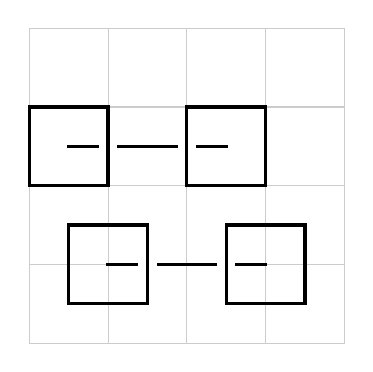
\begin{tikzpicture}
    
    \draw [step=1, line cap = rect, gray!40] (0,0) grid (4,4);
    
    

    \draw[black, line cap=rect, very thick] (0.5,2.5) -- (2.5,2.5) node[pos=0.75, fill=white, anchor=center]{} node[pos=0.25, fill=white, anchor=center]{};

    \draw[black, line cap=rect, very thick] (1,1) -- (3,1) node[pos=0.75, fill=white, anchor=center]{} node[pos=0.25, fill=white, anchor=center]{};
    
    \draw[black, line cap=rect, very thick, xshift=-2cm] (2,2) -- (3,2) -- (3,3) -- (2,3) -- cycle ;

    
    \draw[black, line cap=rect, very thick] (2,2) -- (3,2) -- (3,3) -- (2,3) -- cycle;

    \draw[black, line cap=rect, very thick, xshift=0.5cm, yshift=-1.5cm] (2,2) -- (3,2) -- (3,3) -- (2,3) -- cycle;
    \draw[black, line cap=rect, very thick, xshift=-1.5cm, yshift=-1.5cm] (2,2) -- (3,2) -- (3,3) -- (2,3) -- cycle;

\end{tikzpicture}
\end{document}
